% !TeX TS-program = xelatex

\documentclass{beamer}
%Set the slide theme
%Change to meet your taste
% Madrid, Copenhagen, Berlin, ... works
\usetheme{metropolis}

\usepackage{multicol}

\usepackage{xecolor}
\usepackage{amsmath}
%\usefonttheme[onlymath]{serif} %Change the math font

\usepackage{xepersian}
\settextfont[Path=fonts/]{Parastoo}

%---------------------------------------------------------------------------------
% Seetings to force Beamer works with Xepersian and RTL typesetting
%-------------------------------------------------------------------------------
%\raggedleft

% For right to left lists (itemize and enumerate)
\makeatletter
\newcommand{\RTList}{\raggedleft\rightskip\@totalleftmargin}
\makeatother
% Correct the bullet for RTL texts
\setbeamertemplate{itemize item}{\scriptsize\raise1.25pt%
 \hbox{\donotcoloroutermaths$\blacktriangleleft$}} 

% To force beamer use numbering in captions
\setbeamertemplate{caption}[numbered]{}% Number float-like environments



%---------------------------------------------------------------------------------
\title{
	عنوان پروژه
}
\subtitle{}
\author{پرهام الوانی}
\institute{دانشکده مهندسی کامپیوتر و فناوری اطلاعات}
\date{پاییز ۱۳۹۶}

\begin{document}
\begin{persian}
%------------------------------------------
% Title page
%------------------------------------------
\begin{frame}
\maketitle
\end{frame}

% To adjust the paragraphs in RTL
\everypar{\rightskip\rightmargin}
%-------------------------------------------------------------------------------
\begin{frame}{طرح مساله}
	\begin{itemize}\RTList
		\item سمت کاربر
		\item سمت دیتاسنتر
		\begin{itemize}\RTList
			\item \lr{ETSI GS MANO}
		\end{itemize}
	\end{itemize}
\end{frame}
\begin{frame}{طرح مساله}
	\begin{latin}
		\begin{itemize}
			\item NFVO
			\item VNFM
			\item VIM
		\end{itemize}
	\end{latin}
\end{frame}
\begin{frame}
	\begin{multicols}{3}
		\begin{center}	
			مساله‌ی اول
		\end{center}
	\end{multicols}
	\begin{center}	
		پذیرش زنجیره‌های کارکرد سرویس
		\\
		و مدیریت آن‌ها با استفاده از \lr{VNFM}
	\end{center}
\end{frame}
\begin{frame}{مساله اول}
	\par
	\lr{NFVO} وظیفه‌ی استقرار زنجیره‌های کارکرد سرویس را برعهده دارد.
	همانگونه که در مستند \lr{ETSI} نیز آمده است هر نمونه از کارکردهای مجازی شبکه نیاز دارد
	تحت مدیریت یکی از \lr{VNFM}های موجود در شبکه باشد.
\end{frame}
\begin{frame}{مساله اول}
	\begin{center}\begin{figure}
		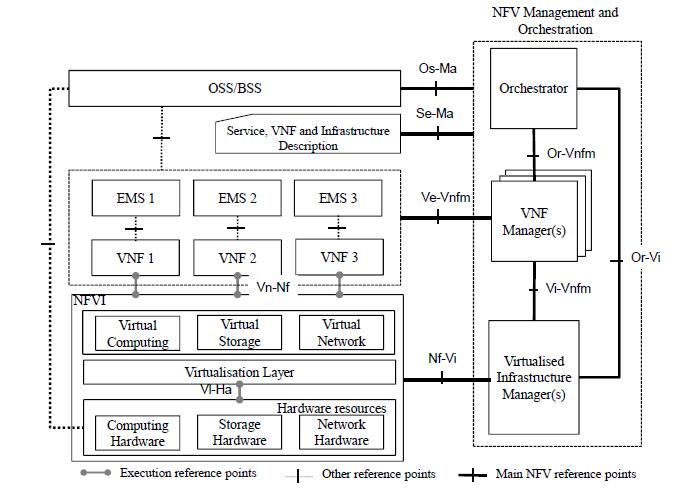
\includegraphics[scale=0.4]{images/nfv-arch.jpg}
		\caption{معماری سطح بالای مجازی‌سازی کارکردهای شبکه}
	\end{figure}\end{center}
\end{frame}
\begin{frame}{مساله اول}
	\par
	یکی از وظایف \lr{VNFM} مانیتور کردن وضعیت و خطاهای نمونه‌ها می‌باشد
	این امر باعث افزایش بار پردازشی \lr{VNFM} می‌گردد
	و از سوی دیگر تحلیل این اطلاعات می‌بایست با تاخیر معقولی صورت پذیرد که این امر
	نیاز به یک بستر ارتباطی مطمئن دارد.
\end{frame}
\begin{frame}{مساله اول}
	\par
	پذیرفتن بیشترین تقاضای زنجیره‌ کارکرد سرویس با در نظر گرفتن نیاز هر نمونه کارکرد مجازی شبکه به یک \lr{VNFM}.
\end{frame}
\begin{frame}{مساله اول}
	\begin{itemize}\RTList
		\item توپولوژی زیرساخت شامل پنهای باند لینک‌ها و ظرفیت \lr{NFVI-PoP}ها موجود است.
		\item n تقاضای زنجیره‌ کارکرد سرویس به صورت کامل و از پیش مشخص شده داریم.
		\item هر تقاضا شامل نوع و تعداد نمونه‌های مجازی و پنهای باند لینک‌های مجازی می‌باشد.
		\item F نوع کارکرد مجازی شبکه تعریف شده است که هر یک مقدار مشخصی از حافظه را مصرف می‌کنند.
		\item تعداد پردازنده‌هایی که به هر نمونه تخصیص می‌یابد با توجه به ترافیک ورودی نمونه مشخص می‌شود.
		\item نمونه‌ها بین زنجیره‌ها به اشتراک گذاشته نمی‌شوند.
	\end{itemize}
\end{frame}
\begin{frame}{مساله اول}
	\begin{itemize}\RTList
		\item محدودیت ظرفیت لینک‌ها
		\item محدودیت توان پردازش سرورهای فیزیکی با توجه به میزان حافظه و تعداد پردازنده‌ها
	\end{itemize}
\end{frame}
\begin{frame}{مساله اول}
	\begin{itemize}\RTList
		\item برای سادگی مساله برای هر زنجیره یک \lr{VNFM} تخصیص می‌دهیم.
		\item \lr{VNFM}ها می‌توانند بین زنجیره به اشتراک گذاشته شوند.
		\item هر نمونه از \lr{VNFM}ها می‌تواند تعداد مشخصی از نمونه‌های کارکرد مجازی شبکه را سرویس دهد. 
		\item برای ارتباط میان هر نمونه از \lr{VNFM}ها و \lr{VNF}ها پهنای باند مشخصی رزرو می‌گردد.
		\item بر روی هر \lr{NFVI-PoP} حداکثر یک نمونه \lr{VNFM} مستقر می‌گردد.
	\end{itemize}
\end{frame}
\begin{frame}{مساله اول}
	\begin{latin}\begin{thebibliography}{9}
		\bibitem{P11}
		Mohammad Abu-Ledbeh, Diala Naboulsi, Roch Glitho, Constant Wette Tchouati.
		\textit{On the Placement of VNF Managers in Large-Scale and Distributed NFV Systems}. 
		IEEE Transactions on Network and Service Management, 2017
	\end{thebibliography}\end{latin}
	\par
	هدف کاهش هزینه‌ی عملیاتی در حالی که تاخیرهای ارتباطی و محدودیت‌های ظرفیت رعایت می‌شوند.
\end{frame}
\begin{frame}{مساله اول}
	\par
	متغیرهای تصمیم‌گیری
	\begin{latin}\begin{tabular}{c p{10cm}}
		$x_h$ & binary variable assuming the value 1 if the $h$th SFC request is accepted; otherwise its value is zero \\
		$y_{wu}$ & the number of VNF instances of type $k$ that are used in server $w \in V_s^{PN}$ \\
		$z^k_{vw}$ & binary variable assuming the value 1 if the VNF node $v \in \cup_{i=1}^{T} V_{i, F}^{SFC}$ is served by the VNF instance of type k in the server $w \in V_s^{PN}$ \\
	\end{tabular}\end{latin}
\end{frame}
\begin{frame}{مساله اول}
	\par
	متغیرهای تصمیم‌گیری
	\begin{latin}\begin{tabular}{c p{10cm}}
		$\bar{y}_w$ & binary varibale assuming the value 1 if VNFM on server $w \in V_s^{PN}$ is used; otherwise its value is zero\\
		$\bar{z}_{hw}$ & binary variable assuming the value 1 if $h$th SFC is assigned to VNFM on server $w \in V_s^{PN}$\\
	\end{tabular}\end{latin}
\end{frame}
\begin{frame}{مساله اول}
	\begin{latin}\begin{align}
	max \sum_{h=1}^Tx_h
	\end{align}\end{latin}
\end{frame}
\begin{frame}{مساله اول}
	\par
	محدودیت حافظه نودها
	\begin{latin}\begin{align}
	\sum_{k=1}^Fy_{wk} memory(k) + \bar{y_w} \bar{memory} \le N_{ram}^{PN}(w)
	\quad
	\forall w \in V_s^{PN}
	\end{align}\end{latin}
	\par
	محدودیت تعداد پردازنده‌های نودها
	\begin{latin}\begin{align}
	\sum_{k=1}^Fy_{wk} core(k) + \bar{y_w} \bar{core} \le N_{core}^{PN}(w)
	\quad
	\forall w \in V_s^{PN}
	\end{align}\end{latin}
\end{frame}
\begin{frame}{مساله اول}
	\par
	یک \lr{VNF} حداکثر یکبار سرویس داده شود.
	\begin{latin}\begin{align}
	\sum_{k=1}^Fy_{wk}\sum_{w \in V_s^{PN}} z_{vw}^{k} \le 1
	\quad
	\forall v \in \cup_{i=1}^T V_{i, F}^{SFC}
	\end{align}\end{latin}
	\par
	اگر \lr{VNF}, \lr{v}
	توسط \lr{VNF instance} نوع \lr{k}
	روی سرور \lr{w} سرویس شود می‌بایست
	\lr{VNF instance} نوع \lr{k}
	روی سرور \lr{w} فعال شود.
	\par
	اشتراک گذاری VNFها پشتیبانی نمی‌گردد.
	\begin{latin}\begin{align}
	\sum_{v \in \cup_{i=1}^T V_{i, F}^{SFC}} z_{vw}^k \le y_{wk}
	\quad
	\forall w \in V_s^{PN}, \forall k \in [1, ..., F]
	\end{align}\end{latin}
\end{frame}
\begin{frame}{مساله اول}
	\par
	اگر تقاضای \lr{h}ام پذیرفته شده باشد
	می‌بایست تمام \lr{VNF node}های آن‌
	سرویس شده باشند.
	\begin{latin}\begin{align}
		x_h \le \sum_{k=1}^{F} \sum_{w \in V_{s}^{PN}} z_{vw}^{k}
		\quad
		\forall v \in V_{h,F}^{SFC}, \forall h \in [1, ..., T]
	\end{align}\end{latin}
\end{frame}
\begin{frame}{مساله اول}
	\par
	اگر تقاضای \lr{h}ام پذیرفته شده باشد
	می‌بایست توسط یک \lr{VNFM} سرویس شده باشد.
	\begin{latin}\begin{align}
		x_h \le \sum_{w \in V_{s}^{PN}} \bar{z}_{hw}
		\quad
		\forall h \in [1, ..., T]
	\end{align}\end{latin}
\end{frame}
\begin{frame}{مساله اول}
	\par
	اگر \lr{SFC}، \lr{i}
	توسط \lr{VNFM} روی سرور \lr{w}
	سرویس شود می‌بایست \lr{VNFM} سرور \lr{w}
	فعال شود.
	\begin{latin}\begin{align}
		\bar{z}_{hw} \le \bar{y}_w
		\quad
		\forall w \in V_{s}^{PN}, \forall h \in [1, ..., T]
	\end{align}\end{latin}
	\par
	محدودیت ظرفیت سرویس‌دهی \lr{VNFM}
	\begin{latin}\begin{align}
		\sum_{i=1}^{T} z_{iw} \le capacity
		\quad
		\forall w \in V_{s}^{PN}
	\end{align}\end{latin}
\end{frame}
\begin{frame}{مساله اول}
	\par
	متغیرهای تصمیم‌گیری
	\begin{latin}\begin{tabular}{c p{10cm}}
		$\tau^{(u,v)}_{ij}$ & binary variable assuming the value 1 if the virual link $(u,v)$ is routed on the physical network link $(i,j)$\\
		$\bar{\tau}^{(u,v)}_{ij}$ & binary variable assuming the value 1 if the managemnt of VNF node $v$ is routed on the physical network link $(i,j)$\\
	\end{tabular}\end{latin}
\end{frame}
\begin{frame}{مساله اول}
	\par
	اگر تقاضای \lr{h}ام پذیرفته شده باشد می‌بایست تمام لینک‌های آن
	مسیریابی شوند.
	\begin{latin}\begin{align}
		x_h \le \sum_{(i,j) \in E^{PN}} \tau_{ij}^{(u,v)}
		\quad
		\forall h \in [1, ..., T], \forall (u,v) \in E_h^{SFC}
	\end{align}\end{latin}
\end{frame}
\begin{frame}{مساله اول}
	\par
	\lr{Flow Conservation}
	\begin{latin}\begin{align}
		\sum_{(i,j) \in E^{PN}} \tau_{ij}^{(u,v)} - \sum_{(j,i) \in E^{PN}} \tau_{ji}^{(u,v)} = \sum_{k=1}^{F} z_{vi}^{k} - \sum_{k=1}^{F} z_{ui}^{k} \nonumber \\
		\forall i \in V_{S}^{PN}, (u,v) \in E_{h}^{SFC}, h \in [1, ..., T]
	\end{align}\end{latin}
\end{frame}
\begin{frame}{مساله اول}
	\par
	اگر تقاضای \lr{h}ام پذیرفته شده باشد
	می‌بایست تمام \lr{VNF}های آن به \lr{VNFM}
	مسیریابی شده باشند.
	\begin{latin}\begin{align}
		x_h \le \sum_{(i,j) \in E^{PN}} \bar{\tau}_{ij}^{v}
		\quad
		\forall h \in [1, ..., T], \forall v \in V_{h,F}^{SFC}
	\end{align}\end{latin}
\end{frame}
\begin{frame}{مساله اول}
	\par
	\lr{Flow Conservation}
	\begin{latin}\begin{align}
		\sum_{(i,j) \in E^{PN}} \bar{\tau}_{ij}^{v} - \sum_{(j,i) \in E^{PN}} \bar{\tau}_{ji}^{v} = \sum_{k=1}^{F} z_{vi}^{k} - \bar{z}_{hi} \nonumber \\
		\forall i \in V_{S}^{PN}, v \in V_{h, F}^{SFC}, h \in [1, ..., T]
	\end{align}\end{latin}
\end{frame}
\begin{frame}{مساله‌ی اول}
	\par
	محدودیت ظرفیت لینک‌ها
	\begin{latin}\begin{align}
		\sum_{v \in \cup_{i=1}^{T} V_{i,F}^{SFC}} \bar{\tau}_{ij}^{v} * \bar{bandwidth} + \sum_{(u,v) \in \cup_{i=1}^{T} E_{i}^{SFC}} \tau_{ij}^{(u,v)} * bandwidth(u,v) \le C_{ij}
	\end{align}\end{latin}
\end{frame}
\begin{frame}
	\begin{multicols}{3}
		\begin{center}	
			مساله‌ی دوم
		\end{center}
	\end{multicols}
	\begin{center}	
		گسترش زنجیره‌های کارکرد سرویس
		\\
		با در نظر گرفتن نقش \lr{VNFM}
	\end{center}
\end{frame}
\begin{frame}{مساله‌ی دوم}
	\par
	مساله از منظر \lr{VNFM} برای \lr{scale} کردن یک \lr{VNF instance}
	زمانی که سیستم به صورت کامل مستقر شده است استفاده می‌گردد.
	این \lr{scale} کردن به دلیل تغییرات ترافیکی در سیستم به وقوع پیوسته است.
\end{frame}
\begin{frame}{مساله‌ی دوم}
	\par
	کمترین هزینه برای اعمال تغییرات بر روی دیتاسنتر.
	در اینجا منظور از هزینه، توان مصرفی سرورها و هزینه‌هایی است که جهت مهاجرت و ساخت نمونه‌ها پرداخت می‌شود.
\end{frame}
\begin{frame}{مساله‌ی دوم}
	\begin{itemize}\RTList
		\item توپولوژی زیرساخت شامل پنهای باند لینک‌ها و ظرفیت \lr{NFVI-PoP}ها موجود است.
		\item وضعیت \lr{NFVI-PoP}ها و نمونه‌هایی که روی آن‌ها مستقر است موجود است.
		\item وضعیت لینک‌های فیزیکی و لینک‌های مجازی که روی آن‌ها قرار دارند موجود است.
		\item تعداد نمونه‌های لازم از پیش مشخص است.
		\item با ایجاد نمونه‌های جدید ترافیک ورودی و خروجی نمونه‌ی اولیه بین نمونه‌های جدید تقسیم می‌گردد.
		\item تنها در مورد یک نمونه از یک زجیره بحث می‌گردد.
	\end{itemize}
\end{frame}
\begin{frame}{مساله‌ی دوم}
	\begin{itemize}\RTList
		\item نمونه‌ها به صورت عمودی مقیاس‌پذیر نیستند.
		\item محدودیت توان پردازشی سرورهای فیزیکی با توجه به تعداد پردازنده‌ها
		\begin{itemize}\RTList
			\item هزینه‌ی ساخت نمونه
			\item هزینه‌ی مهاجرت نمونه (\lr{hot migration}) بر اساس جابجایی حافظه
			\item هزینه‌ی روشن کردن سرور جدید
		\end{itemize}
	\end{itemize}
\end{frame}
\begin{frame}{مساله‌ی دوم}
	\begin{latin}\begin{thebibliography}{9}
		\bibitem{P21}
		Vincenzo Eramo, Emanuele Miucci, Mostafa Ammar.
		\textit{An Approach for Service Function Chain Routing and Virtual Function Network Intance Migration in Network Function Virtualization Architecture}. 
		IEEE Transactions on Networking, 2017
	\end{thebibliography}\end{latin}
	\par
	کاهش توان مصرفی در یک ترافیک \lr{cycle-stationary}
	با مهاجرت و مقیاس‌دهی عمودی نمونه‌ها در وضعیت‌های ترافیکی مختلف
\end{frame}
\begin{frame}{مساله‌ی دوم}
	\par
	متغیرهای تصمیم‌گیری
	\begin{latin}\begin{tabular}{c p{10cm}}
		$y_w$ & the number of VNF instances that are run on server w\\
		$\tau_{ij}$ & the number of virtual links that are routed on physical link $(i,j)$\\
		$P_w$ & binary variable assuming the value 1 if server $w$ has at least one instance of target VNF or has VNFM\\
		$\bar{y}_w$ & the number of VNF instances that are connected to VNFM on server $w$\\	
		$\bar{\tau}$ & the number of management virtual links that are routed on physical link $(i,j)$\\
	\end{tabular}\end{latin}
\end{frame}
\begin{frame}{مساله‌ی دوم}
	\par
	محدودیت حافظه نودها
	\begin{latin}\begin{align}
		y_{w} * memory \le N_{ram}^{PN}(w)
		\quad
		\forall w \in V_s^{PN}
		\end{align}\end{latin}
	\par
	محدودیت تعداد پردازنده‌های نودها
	\begin{latin}\begin{align}
		y_{w} * core \le N_{core}^{PN}(w)
		\quad
		\forall w \in V_s^{PN}
	\end{align}\end{latin}
	\par
	محدودیت ظرفیت \lr{VNFM}
	\begin{latin}\begin{align}
		\bar{y}_w \le capacity
	\end{align}\end{latin}
\end{frame}
\begin{frame}{مساله‌ی دوم}
	\par
	می‌بایست تمام نمونه‌ها سرویس شده باشند
	\begin{latin}\begin{align}
		\sum_{w in V_{S}^{PN}} y_w \le V\\
		\sum_{w in V_{S}^{PN}} \bar{y}_w \le V
	\end{align}\end{latin}
	\par
	اگر نمونه روی سرور \lr{w} باشد می‌بایست آن سرور روشن باشد.
	\begin{latin}\begin{align}
		y_w \le M * P_w
		\quad
		\forall w \in V_{s}^{PN}\\
		\bar{y}_w \le M * P_w
		\quad
		\forall w \in V_{s}^{PN}
	\end{align}\end{latin}
\end{frame}
\begin{frame}{مساله‌ی دوم}
	\par
	\lr{Flow Conservation}
	\begin{latin}\begin{align}
		\sum_{(i,j) \in E^{PN}} \tau_{ij} - \sum_{(j,i) \in E^{PN}} \tau_{ji} = is_source(i) - y_i \nonumber \\
		\forall i \in V_{S}^{PN}
	\end{align}\end{latin}
	\begin{latin}\begin{align}
		\sum_{(i,j) \in E^{PN}} \tau_{ij} - \sum_{(j,i) \in E^{PN}} \tau_{ji} = y_i - is_destination(i) \nonumber \\
		\forall i \in V_{S}^{PN}
	\end{align}\end{latin}
\end{frame}
\begin{frame}{مساله‌ی دوم}
	\par
	\lr{Flow Conservation}
	\begin{latin}\begin{align}
		\sum_{(i,j) \in E^{PN}} \bar{\tau}_{ij} - \sum_{(j,i) \in E^{PN}} \bar{\tau}_{ji} = y_i - \bar{y}_i \nonumber \\
		\forall i \in V_{S}^{PN}
	\end{align}\end{latin}
\end{frame}
\begin{frame}{مساله‌ی دوم}
	\par
	محدودیت ظرفیت لینک‌ها	
	\begin{latin}\begin{align}
		\bar{\tau}_{ij} * \bar{bandwidth} + \tau_{ij} * bandwidth \le C_{ij}
	\end{align}\end{latin}
\end{frame}
\begin{frame}{مساله‌ی سوم}
	\par
	مساله از منظر \lr{NFVO} برای به روزرسانی یک \lr{VNF-FG}
	مطرح شده است.
\end{frame}
\begin{frame}
	\par
	کمترین هزینه (تغییرات) برای به روزرسانی یک \lr{VNF-FG}
	در یک سیستم مستقر شده
\end{frame}
\begin{frame}
	\begin{itemize}\RTList
		\item توپولوژی زیرساخت شامل پنهای باند لینک‌ها و ظرفیت \lr{NFVI-PoP}ها موجود است.
		\item وضعیت \lr{NFVI-PoP}ها و نمونه‌هایی که روی آن‌ها مستقر است موجود است.
		\item وضعیت لینک‌های فیزیکی و لینک‌های مجازی که روی آن‌ها قرار دارند موجود است.
		\item تغییرات شامل اضافه و کم شدن نمونه‌ها و لینک‌ها می‌باشد.
		\begin{itemize}\RTList
			\item هزینه‌ی ساخت نمونه
			\item هزینه‌ی مهاجرت نمونه (\lr{hot migration}) بر اساس جابجایی حافظه
			\item هزینه‌ی روشن کردن سرور جدید
		\end{itemize}
	\end{itemize}
\end{frame}
\end{persian}
\end{document}
